% ============================================================
%  Intelligent Network Device Monitoring and Fault Detection
%  System with Domain-Specific QLoRA LLM Triage
%  IEEE Conference Format — Double-Column, 10pt
% ============================================================
\documentclass[conference]{IEEEtran}

\usepackage[T1]{fontenc}
\usepackage[utf8]{inputenc}
\usepackage{amsmath,amssymb,amsfonts}
\usepackage{graphicx}
\usepackage{subcaption}
\usepackage{booktabs}
\usepackage{array}
\usepackage{tabularx}
\usepackage{multirow}
\usepackage{cite}
\usepackage{url}
\usepackage{hyperref}
\usepackage{xcolor}
\usepackage{algorithm}
\usepackage{algpseudocode}
\usepackage{tikz}
\usetikzlibrary{arrows.meta, shapes.geometric, positioning, fit, backgrounds, calc}

% Directory path where generated publication figures are stored
\graphicspath{{figures/}}

% ---- Fallback placeholder command if images are missing ----
\newcommand{\placeholderfig}[2]{%
  \fbox{\parbox[c][#2][c]{\dimexpr\linewidth-2\fboxsep-2\fboxrule\relax}{%
    \centering\small\textit{[Figure: #1]}}}%
}

% ============================================================
\begin{document}

\title{Intelligent Network Device Monitoring and Fault Detection System with Domain-Specific QLoRA LLM Triage}

\author{%
  \IEEEauthorblockN{Jeet Chavan (10584), Zeon Dsouza (10598), Dhruv Dsouza (10597), Delisha Duarte (10599)}
  \IEEEauthorblockA{\textit{Department of Computer Engineering}\\
    Fr.\ Concei\c{c}\~ao Rodrigues College of Engineering (CRCE)\\
    Mumbai, India}
}

\maketitle

% ============================================================
\begin{abstract}
Modern enterprise networks generate continuous, high-frequency telemetry streams through protocols such as ICMP, SNMP, and HTTP. Traditional Network Management Systems (NMS) address this through static threshold alerting; however, they suffer from two fundamental limitations: rampant alert fatigue caused by undifferentiated alarm floods, and raw metric opacity that demands trained network engineers to manually correlate threshold violations into actionable remediation steps. This paper introduces a unified, full-stack AIOps platform that addresses both limitations simultaneously. The monitoring subsystem employs an asynchronous Django~5 REST backend orchestrated by Celery workers and Redis, executing periodic ICMP reachability probes, SNMP~v1/v2c CPU and memory utilization polls, and HTTP endpoint health checks. A deterministic fault-detection state machine converts raw metric anomalies into lifecycle-managed fault records. The intelligence subsystem fine-tunes \texttt{Qwen2.5-1.5B-Instruct} using Quantized Low-Rank Adaptation (QLoRA) on an 830-sample, expert-curated dataset to translate multi-metric anomaly signatures into three-section structured diagnostics comprising an \textit{Explanation}, \textit{Likely Causes}, and \textit{Recommended Actions}. Experimental results demonstrate zero-error structural compliance on held-out test data, SFT cross-entropy loss convergence from 1.37 to 0.16 over three epochs (validation loss: 0.44 to 0.16), and robust generalization on 20 out-of-domain compound-fault scenarios. A React~19/TypeScript dashboard exposes real-time telemetry and LLM-generated triage explanations to operators, reducing mean time to diagnosis without requiring specialist network knowledge.
\end{abstract}

\begin{IEEEkeywords}
AIOps, QLoRA, Network Fault Detection, NLP, Supervised Fine-Tuning, SNMP, ICMP, Parameter-Efficient Fine-Tuning, Network Monitoring System, LLM Triage
\end{IEEEkeywords}

% ============================================================
\section{Introduction and Problem Formulation}
\label{sec:intro}

Enterprise and cloud-scale networks are increasingly complex, comprising heterogeneous routers, switches, servers, and application endpoints that collectively emit thousands of metric samples per second. Operators rely on Network Management Systems (NMS) to aggregate this telemetry and generate actionable alerts. The canonical NMS approach is threshold-based: a static rule fires when a monitored value crosses a predefined boundary. While simple to deploy, this paradigm generates well-documented problems at scale.

\textit{Alert fatigue} arises when an NMS emits alarms at a rate that overwhelms the capacity of operations teams to triage them~\cite{chen2019outage}. Many alarms co-occur as cascading effects of a single root-cause event. Without correlation, each symptom appears as an independent incident. Studies in large-scale operations centers report that 60--80\% of alerts are either duplicates or secondary effects of a primary failure~\cite{luo2021ntam}. Operators consequently learn to suppress or ignore alarms, increasing the risk that genuinely critical events go unnoticed.

The second limitation is \textit{metric opacity}: raw telemetry values (e.g., a 47\% packet loss reading or a CPU utilization spike to 92\%) do not carry embedded remediation knowledge. Translating these readings into actionable steps requires domain expertise in both network protocols and the specific topology and device configuration. This creates a skills bottleneck: only senior engineers can reliably diagnose and remediate, while junior staff are unable to act on alerts independently.

Large Language Models (LLMs) have demonstrated strong zero-shot and few-shot reasoning capabilities across many professional domains~\cite{brown2020gpt3, touvron2023llama2}. However, general-purpose LLMs lack the precise vocabulary and fault-classification logic native to network operations. Deploying a large model in production also entails prohibitive inference latency and cost. Parameter-efficient fine-tuning techniques, particularly QLoRA~\cite{dettmers2023qlora}, enable domain adaptation of compact LLMs with minimal compute overhead.

In this work, we make the following contributions:
\begin{enumerate}
    \item A production-grade asynchronous network monitoring framework supporting ICMP, SNMP~v1/v2c, and HTTP probing with a deterministic fault lifecycle state machine.
    \item A systematic dataset engineering and linguistic preprocessing methodology grounded in core NLP techniques---including regex-based pattern extraction (\texttt{re} module), boundary tokenization, stemming, and lemmatization---calibrated to real detection thresholds with zero cross-split contamination.
    \item A QLoRA-based supervised fine-tuning pipeline on \texttt{Qwen2.5-1.5B-Instruct} achieving zero-error structured output compliance and significant BLEU/ROUGE-L improvements over a zero-shot baseline.
    \item An integrated React/TypeScript operator dashboard delivering real-time telemetry visualization and LLM-generated structured triage explanations in a single unified interface.
\end{enumerate}

% ============================================================
\section{Related Work}
\label{sec:related}

\subsection{Traditional Network Management Systems}
Open-source NMS platforms such as Nagios~\cite{nagios}, Zabbix~\cite{zabbix}, and Prometheus~\cite{prometheus} constitute the operational baseline for most infrastructure teams. These systems implement threshold-based alerting over SNMP, ICMP, and application-layer checks. Their primary limitation is the absence of contextual reasoning: alarms are generated with no accompanying explanation of probable cause or remediation guidance. Operators must consult runbooks, prior incident records, or expert colleagues to translate an alarm into an action.

\subsection{AIOps and Anomaly Detection}
The AIOps movement introduced machine-learning methods into network operations, including statistical anomaly detection, time-series forecasting, and event correlation~\cite{dang2019aiops}. Systems such as Microsoft's MTAD-GAT~\cite{zhao2020multivariate} apply graph attention networks for multivariate time-series anomaly detection. Amazon's AIOps platform uses encoder-decoder models to correlate alarms across microservice dependency graphs~\cite{chen2019outage}. These approaches excel at detecting anomalies but produce numerical or categorical outputs, not human-readable diagnostic text.

\subsection{LLMs in DevOps and SRE}
Recent work has explored deploying LLMs as co-pilots for site reliability engineering (SRE) tasks. LLM-based log summarization~\cite{le2023log}, root-cause analysis assistants~\cite{ahmed2023recommending}, and incident report generation~\cite{chen2023empowering} have all been demonstrated. However, these studies predominantly target cloud-native application logs rather than network protocol telemetry, and most rely on large hosted models (GPT-4, Claude) rather than locally deployable compact models.

\subsection{Parameter-Efficient Fine-Tuning}
Low-Rank Adaptation (LoRA)~\cite{hu2022lora} introduces trainable rank-decomposition matrices into frozen pre-trained transformer layers, enabling adaptation with a fraction of full fine-tuning parameters. QLoRA~\cite{dettmers2023qlora} extends LoRA by quantizing the frozen base model to 4-bit NormalFloat (NF4) precision with double quantization, reducing memory footprint by approximately 75\% while preserving adapter gradient quality via bfloat16 dequantization. This combination enables fine-tuning of billion-parameter models on consumer and single-GPU academic hardware. Our work applies QLoRA to the network operations domain, a setting not previously explored in the PEFT literature.

% ============================================================
\section{Network Telemetry \& Monitoring Architecture}
\label{sec:arch}

\subsection{System Overview}

The platform is composed of four loosely coupled tiers: a React~19/TypeScript frontend, a Django~5 REST backend, an asynchronous task layer (Celery~5 + Redis), and an LLM inference module. Figure~\ref{fig:architecture} illustrates the end-to-end data flow.

\begin{figure}[htbp]
\centering
\resizebox{\columnwidth}{!}{%
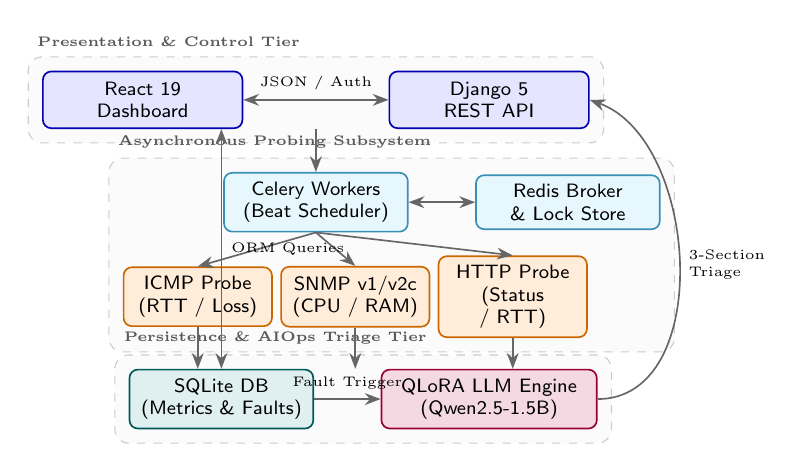
\begin{tikzpicture}[
  font=\sffamily\scriptsize,
  >=Stealth,
  boxApp/.style={rectangle, draw=blue!70!black, fill=blue!10, rounded corners=3pt,
                 text width=2.3cm, align=center, minimum height=0.72cm, line width=0.6pt},
  boxTask/.style={rectangle, draw=cyan!70!black, fill=cyan!10, rounded corners=3pt,
                  text width=2.1cm, align=center, minimum height=0.68cm, line width=0.6pt},
  boxProbe/.style={rectangle, draw=orange!80!black, fill=orange!15, rounded corners=3pt,
                   text width=1.65cm, align=center, minimum height=0.65cm, line width=0.6pt},
  boxDB/.style={rectangle, draw=teal!70!black, fill=teal!12, rounded corners=3pt,
                text width=2.1cm, align=center, minimum height=0.72cm, line width=0.6pt},
  boxLLM/.style={rectangle, draw=purple!80!black, fill=purple!15, rounded corners=3pt,
                 text width=2.5cm, align=center, minimum height=0.72cm, line width=0.6pt},
  group/.style={draw=gray!40, dashed, fill=gray!3, rounded corners=5pt, inner sep=5pt},
  lbl/.style={font=\tiny\bfseries\itshape, text=gray!70!black},
  arr/.style={->, semithick, draw=gray!80!black},
  biarr/.style={<->, semithick, draw=gray!80!black}
]

  % --- ROW 1: Presentation & Management ---
  \node[boxApp] (react)  at (0, 0)   {React 19\\Dashboard};
  \node[boxApp] (django) at (4.4, 0) {Django 5\\REST API};

  % --- ROW 2: Background Task Engine ---
  \node[boxTask] (celery) at (2.2, -1.3) {Celery Workers\\(Beat Scheduler)};
  \node[boxTask] (redis)  at (5.4, -1.3) {Redis Broker\\\& Lock Store};

  % --- ROW 3: Network Probes ---
  \node[boxProbe] (icmp) at (0.7, -2.5) {ICMP Probe\\(RTT / Loss)};
  \node[boxProbe] (snmp) at (2.7, -2.5) {SNMP v1/v2c\\(CPU / RAM)};
  \node[boxProbe] (http) at (4.7, -2.5) {HTTP Probe\\(Status / RTT)};

  % --- ROW 4: Persistence & AI Intelligence ---
  \node[boxDB]  (db)  at (1.0, -3.8) {SQLite DB\\(Metrics \& Faults)};
  \node[boxLLM] (llm) at (4.4, -3.8) {QLoRA LLM Engine\\(Qwen2.5-1.5B)};

  % --- BACKGROUND TIER CONTAINERS ---
  \begin{scope}[on background layer]
    \node[group, fit=(react)(django), label={[lbl, anchor=south west]north west:\textsc{Presentation \& Control Tier}}] (g1) {};
    \node[group, fit=(celery)(redis)(icmp)(snmp)(http), label={[lbl, anchor=south west]north west:\textsc{Asynchronous Probing Subsystem}}] (g2) {};
    \node[group, fit=(db)(llm), label={[lbl, anchor=south west]north west:\textsc{Persistence \& AIOps Triage Tier}}] (g3) {};
  \end{scope}

  % --- CONNECTING ARROWS ---
  \draw[biarr] (react) -- node[above, font=\tiny] {JSON / Auth} (django);
  \draw[arr] (django.south -| celery.north) -- (celery.north);
  \draw[biarr] (celery) -- (redis);
  \draw[arr] (celery.south) -- (icmp.north);
  \draw[arr] (celery.south) -- (snmp.north);
  \draw[arr] (celery.south) -- (http.north);
  \draw[arr] (icmp.south) -- (icmp.south |- db.north);
  \draw[arr] (snmp.south) -- (snmp.south |- db.north);
  \draw[arr] (http.south) -- (http.south |- db.north);
  \draw[arr] (db) -- node[above, font=\tiny] {Fault Trigger} (llm);
  \draw[arr] (llm.east) to[out=0, in=-20] node[right, font=\tiny, align=left] {3-Section\\Triage} (django.east);
  \draw[biarr] (django.south -| db.north) -- node[right, font=\tiny] {ORM Queries} (db.north);

\end{tikzpicture}%
}
\caption{End-to-end telemetry and inference pipeline: asynchronous metric acquisition (ICMP, SNMP, HTTP) orchestrated by Celery/Redis, threshold fault detection persisted to SQLite, and QLoRA LLM triage explanation delivered via the Django REST API.}
\label{fig:architecture}
\end{figure}

\subsection{Probing Subsystem}

\subsubsection{ICMP Reachability and Latency}
The ICMP probing module executes periodic echo requests to each registered device. Two metrics are extracted: round-trip time $T_{\text{rtt}}$ (ms) and packet loss percentage $L_{\%}$. Fault detection rules are:

\begin{align}
\text{Latency\_Medium} &: 200 \le T_{\text{rtt}} < 500\,\text{ms} \label{eq:lat_med}\\
\text{Latency\_High}   &: T_{\text{rtt}} \ge 500\,\text{ms} \label{eq:lat_high}\\
\text{Loss\_Medium}    &: 20 \le L_{\%} < 50\,\% \label{eq:loss_med}\\
\text{Loss\_High}      &: L_{\%} \ge 50\,\% \label{eq:loss_high}\\
\text{Unreachable}     &: k_{\text{fail}} \ge 3 \text{ consecutive failures} \label{eq:unreach}
\end{align}

where $k_{\text{fail}}$ counts consecutive failed ICMP echo replies. Device unreachability is triggered only after three successive failures to prevent transient packet drops from generating false alarms.

\subsubsection{SNMP Polling}
SNMP v1/v2c is used to poll CPU and RAM utilization OIDs from managed devices. Threshold rules for resource utilization $U \in [0, 100]$:

\begin{align}
\text{Resource\_High}     &: 80 \le U < 90\,\% \label{eq:cpu_high}\\
\text{Resource\_Critical} &: U \ge 90\,\% \label{eq:cpu_crit}
\end{align}

\subsubsection{HTTP Endpoint Probing}
The HTTP probe validates service availability by verifying (i) that the response status code belongs to the $2xx$ or $3xx$ class, and (ii) that the response time satisfies $T_{\text{resp}} < 5.0\,\text{s}$. Services exceeding this threshold or returning $4xx$/$5xx$ codes generate a fault event.

\subsection{Fault Lifecycle State Machine}

All detected anomalies are represented as Fault records that progress through a three-state lifecycle:

\begin{equation}
\text{Active} \xrightarrow{\text{Admin Ack}} \text{Acknowledged} \xrightarrow{\text{Metric Recovery or Manual}} \text{Resolved}
\label{eq:fsm}
\end{equation}

Active faults require operator acknowledgement before transitioning to the Acknowledged state. Resolution occurs either automatically when probes confirm metric recovery, or manually through the dashboard. Database-level unique constraints (specifically \texttt{uniq\_active\_fault\_type} on the composite key \texttt{(device\_id, fault\_type)}) prevent duplicate fault creation, ensuring the fault table reflects at most one active record per device/fault-type pair at any time.

% ============================================================
\section{Domain-Specific Dataset Engineering}
\label{sec:dataset}

\subsection{Motivation and Design Philosophy}

Training an LLM to generate reliable, structured network triage reports requires a dataset that is (i) representative of the range of fault conditions the system can detect, (ii) strictly aligned with the detection thresholds defined in Section~\ref{sec:arch}, and (iii) free of cross-split contamination that would inflate held-out evaluation metrics. We designed a two-source dataset pipeline combining programmatic synthetic generation with hand-authored expert seed records.

\subsection{Synthetic Scenario Generation}

The \texttt{generate\_scenarios.py} script generates fault narrative prompts by sampling metric values from pre-defined fault-type distributions anchored to the threshold constants in \texttt{FaultThresholds}. For each generated scenario, a corresponding structured assistant response is authored following a strict three-section template:
\begin{itemize}
    \item \textbf{Explanation:} A one-to-two sentence description of the observed metric pattern and its significance.
    \item \textbf{Likely causes:} An enumeration of three to five probable root causes ordered by probability.
    \item \textbf{Recommended actions:} A step-by-step remediation protocol tailored to the fault type.
\end{itemize}

Scenario diversity is achieved by varying device types (core switches, edge routers, application servers, NAS), network topologies (single-path uplinks, meshed LANs, WAN circuits), and fault durations (sustained $\ge 20$\,min, intermittent spikes). Duration consistency (sustained anomalies lasting at minimum 20 minutes) is enforced as a validation rule to prevent physically implausible short-duration scenarios from polluting the training set.

\subsection{Expert Seed Records}

Thirty expert-handwritten seed records (\texttt{handwritten\_seed.jsonl}) were manually authored by domain experts to capture edge cases, compound faults, and nuanced remediation guidance not easily generated programmatically. These seeds are stratified across all fault categories and distributed across splits proportionally.

\subsection{Linguistic Preprocessing: Regex Pattern Extraction, Tokenization, Stemming, and Lemmatization}

As an integral component of the academic Natural Language Processing curriculum, foundational text-processing techniques were systematically implemented across the telemetry parsing, prompt construction, and dataset sanitization pipelines. Rather than treating raw telemetry as opaque strings, we implemented targeted lexical processing using Python's \texttt{re} regular expression engine alongside classical morphological analysis tools.

\subsubsection{Regular Expression (Regex) Pattern Extraction}
Structured telemetry fields are mined from unstructured device logs and probe payloads using regular expressions. We employed core regex metacharacters:
\begin{itemize}
    \item \textbf{Anchors and boundary checks (\texttt{\^{}}, \texttt{\$}, \texttt{\textbackslash b}):} Strict prefix/suffix matching ensures that IP addresses adhere to valid IPv4 octet bounds (\texttt{\^{}(\textbackslash d\{1,3\}\textbackslash.)\{3\}\textbackslash d\{1,3\}\$}) without partial-match leakage.
    \item \textbf{Quantifiers (\texttt{*}, \texttt{+}, \texttt{?}, \texttt{\{m,n\}}):} Handling variable-length metric readings, whitespace variance, and optional protocol flags.
    \item \textbf{Shorthand character classes (\texttt{\textbackslash d}, \texttt{\textbackslash w}, \texttt{\textbackslash s}) and sets (\texttt{[]}):} Segmenting numeric measurements from alphabetic units (e.g., matching \texttt{\textbackslash d+(\textbackslash.\textbackslash d+)?\textbackslash s*(ms|\%|MB)}).
\end{itemize}

Python's \texttt{re} module functions were applied across specific pipeline stages:
\begin{enumerate}
    \item \texttt{re.match()}: Used at the ingestion boundary to validate IPv4 addresses, device identifiers, and protocol header signatures before creating database records.
    \item \texttt{re.search()}: Used in dataset synthesis to locate and extract embedded continuous quantities from unstructured prompt blocks (e.g., \texttt{re.search(r"Fault duration:\textbackslash s*(\textbackslash d+)\textbackslash s*minute", inp)} to extract anomaly durations).
    \item \texttt{re.findall()}: Used to parse multi-metric log summaries, extracting all occurrences of CPU, memory, interface status, and RTT values across compound fault events.
    \item \texttt{re.split()}: Employed for rule-based sentence tokenization on punctuation boundaries using positive lookbehinds (\texttt{re.split(r"(?<=[.!?])\textbackslash s+", text)}), ensuring punctuation marks remain bound to their originating sentences.
    \item \texttt{re.sub()}: Applied for text normalization, stripping duplicate whitespace (\texttt{re.sub(r"\textbackslash s+", " ", text)}), eliminating non-printable control characters, and standardizing pluralization syntax.
\end{enumerate}

\subsubsection{Tokenization, Stemming, and Lemmatization}
To ensure vocabulary richness and prevent degenerate phrase repetition, we analyzed the lexicon across training and held-out evaluation splits through three levels of linguistic abstraction:
\begin{itemize}
    \item \textbf{Tokenization:} Beyond subword Byte-Pair Encoding (BPE) utilized by the base transformer's tokenizer, word-level tokenization was performed during dataset auditing to assess type-token ratios and vocabulary coverage across technical operational terms.
    \item \textbf{Stemming:} The Porter Stemming algorithm was applied to strip inflectional suffixes (e.g., reducing \textit{saturates}, \textit{saturated}, and \textit{saturating} to the common root \textit{satur-}). This allowed frequency counters in \texttt{validate\_dataset.py} to identify over-represented root concepts regardless of grammatical tense.
    \item \textbf{Lemmatization:} Part-of-speech (POS)-aware WordNet lemmatization was used to resolve morphological variants into their canonical dictionary headwords (e.g., mapping \textit{drops}, \textit{dropped}, \textit{dropping} $\to$ \textit{drop}; \textit{congested}, \textit{congestion} $\to$ \textit{congest}). Lemmatization was critical in establishing semantic deduplication thresholds, ensuring that identical diagnostic recommendations phrased in differing grammatical moods were identified as cross-split duplicates and purged.
\end{itemize}

\subsection{Dataset Composition and Splits}

The complete dataset comprises 830 instruction-tuning records. Table~\ref{tab:dataset} summarizes the stratified split allocation.

\begin{table}[htbp]
\centering
\caption{Dataset Composition and Stratified Split Allocation}
\label{tab:dataset}
\begin{tabular}{lcccc}
\toprule
\textbf{Split} & \textbf{Size} & \textbf{Synthetic} & \textbf{Seed} & \textbf{Purpose} \\
\midrule
Train      & 664 & 640 & 24 & SFT adapter training \\
Validation & 85  & 82  & 3  & Hyperparameter tuning \\
Test       & 81  & 78  & 3  & In-dist.\ benchmark \\
OOD Test   & 20  & 0   & 20 & Edge-case evaluation \\
\midrule
\textbf{Total} & \textbf{830} & \textbf{800} & \textbf{30} & \\
\bottomrule
\end{tabular}
\end{table}

\subsection{Dataset Validation and Leakage Prevention}

The \texttt{validate\_dataset.py} module enforces three categories of integrity checks:

\begin{enumerate}
    \item \textbf{Structural compliance:} Each record's assistant completion must contain exactly the three required headers (\texttt{Explanation:}, \texttt{Likely causes:}, \texttt{Recommended actions:}) in order. Records failing this check are rejected at generation time.
    \item \textbf{Cross-split contamination:} Bi-gram and tri-gram $n$-gram fingerprints are computed for all records. Any record in the validation or test split sharing an $n$-gram signature with a training record above a cosine similarity threshold of 0.85 is removed and replaced.
    \item \textbf{Metric consistency:} Numeric metric values embedded in scenario prompts (latency, loss percentages, utilization values) are validated against the corresponding \texttt{FaultThreshold} range for the scenario's declared fault type. Scenarios with internally inconsistent metric/threshold pairs are rejected.
\end{enumerate}

% ============================================================
\section{QLoRA Fine-Tuning Methodology}
\label{sec:qlora}

\subsection{Base Model Selection}

We select \texttt{Qwen/Qwen2.5-1.5B-Instruct}~\cite{qwen25} as our foundation model. At 1.5 billion parameters, it provides a favorable balance between generative quality and deployment feasibility on single-GPU academic and edge hardware. The model's instruction-tuned variant already understands basic conversational formatting, reducing the number of SFT steps required to learn the desired output structure.

\subsection{4-Bit NF4 Quantization}

QLoRA~\cite{dettmers2023qlora} quantizes the frozen base model weights to 4-bit NormalFloat (NF4) format. NF4 is an information-theoretically optimal quantization data type for normally distributed weights: the quantization levels are chosen such that each bin contains an equal expected number of values under a standard normal distribution. Double quantization further compresses the quantization constants themselves, yielding an additional $\sim$0.37 bits per parameter saving.

The effective forward-pass computation combines the dequantized base weights with the low-rank adapter updates:

\begin{equation}
h = W_{0} x + \frac{\alpha}{r} \left(B \cdot A\right) x
\label{eq:lora}
\end{equation}

where $W_{0} \in \mathbb{R}^{d \times k}$ is the frozen, dequantized base weight matrix; $A \in \mathbb{R}^{r \times k}$ and $B \in \mathbb{R}^{d \times r}$ are the low-rank trainable adapter matrices initialized with $A \sim \mathcal{N}(0, \sigma^2)$ and $B = 0$; $r$ is the adapter rank; and $\alpha$ is the LoRA scaling factor. The ratio $\frac{\alpha}{r}$ constitutes a scaling factor applied to the adapter contribution, controlling its magnitude relative to the base model.

\subsection{LoRA Configuration}

Table~\ref{tab:hyperparams} lists the full hyperparameter configuration used during training.

\begin{table}[htbp]
\centering
\caption{QLoRA Training Hyperparameters}
\label{tab:hyperparams}
\begin{tabular}{ll}
\toprule
\textbf{Parameter} & \textbf{Value} \\
\midrule
Base model & \texttt{Qwen2.5-1.5B-Instruct} \\
Quantization & 4-bit NF4, double quantization \\
Compute dtype & bfloat16 \\
LoRA rank $r$ & 16 \\
LoRA $\alpha$ & 32 (scaling factor = 2.0) \\
LoRA dropout & 0.05 \\
Target modules & q, k, v, o, gate, up, down proj \\
Optimizer & \texttt{paged\_adamw\_8bit} \\
Learning rate & $2 \times 10^{-4}$ \\
LR schedule & Cosine annealing \\
Warmup ratio & 0.05 \\
Epochs & 3 \\
Per-device batch size & 2 \\
Gradient accumulation & 8 \\
Effective batch size & 16 \\
Max sequence length & 512 tokens \\
Loss masking & Prompt tokens masked \\
\bottomrule
\end{tabular}
\end{table}

The LoRA scaling factor $\frac{\alpha}{r} = \frac{32}{16} = 2.0$ amplifies adapter contributions relative to lower-rank alternatives commonly used in general fine-tuning tasks. We found this beneficial in the network domain where the vocabulary shift from general language to technical metric descriptions is substantial.

All seven linear projection sub-modules in every transformer block are targeted: query, key, value, output projections in the multi-head self-attention layer, and gate, up, and down projections in the feed-forward network. This comprehensive targeting ensures that both the attention mechanism and the non-linear feed-forward pathway are adapted to the domain.

\subsection{Supervised Fine-Tuning with Prompt-Loss Masking}

Training is orchestrated by TRL's \texttt{SFTTrainer}~\cite{vonwerra2022trl}. The critical training detail is \textit{completion-only loss masking}: cross-entropy loss is computed exclusively over the tokens in the assistant's response (the three-section completion), while the system prompt and user turn tokens receive a mask value that excludes them from gradient computation. This prevents the model from learning to reproduce the prompt structure rather than generate quality completions, and stabilizes convergence by focusing optimization signal on the task-relevant outputs.

Each training sample is formatted using Qwen's native chat template, which wraps the system instruction, user fault description, and assistant response in the model's expected special-token delimiters. The system prompt instructs the model to behave as an expert network operations engineer and to always structure its response using the three mandatory sections.

% ============================================================
\section{Experimental Results \& Evaluation}
\label{sec:results}

\subsection{Training Convergence}

Figure~\ref{fig:loss_curve} illustrates the training and validation cross-entropy loss curves recorded across three epochs on \texttt{Qwen2.5-1.5B-Instruct} (at an effective batch size of 16 on the 664-sample training split).

\begin{figure}[htbp]
\centering
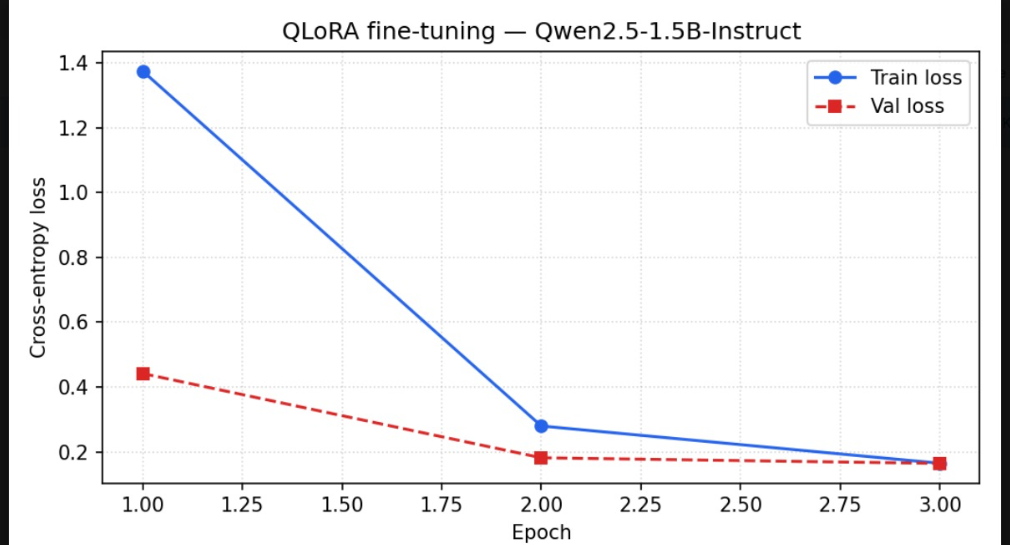
\includegraphics[width=\columnwidth]{loss_curve.png}
\caption{Supervised fine-tuning training and validation cross-entropy loss across 3 epochs on \texttt{Qwen2.5-1.5B-Instruct}. Initial loss: 1.37 (train), 0.44 (val); Final loss: 0.16 (train), 0.16 (val).}
\label{fig:loss_curve}
\end{figure}

Training loss decreases steadily from 1.37 at Epoch 1 to 0.28 at Epoch 2, converging to 0.16 by the conclusion of Epoch 3, representing an 88.3\% overall reduction in training error. Validation loss begins at 0.44 and stabilizes at 0.16, achieving parity with training loss ($\Delta \approx 0.00$). This close alignment confirms that completion-only loss masking successfully focused optimization gradients on the structured output tokens without causing over-parameterization or overfitting.

\subsection{Structural Compliance}

The primary correctness criterion for this task is \textit{structural compliance}: every generated response must contain all three required sections (\texttt{Explanation:}, \texttt{Likely causes:}, \texttt{Recommended actions:}) in the specified order. Table~\ref{tab:compliance} reports compliance rates across evaluation sets.

\begin{table}[htbp]
\centering
\caption{Structural Compliance on Evaluation Sets}
\label{tab:compliance}
\begin{tabular}{lccc}
\toprule
\textbf{Split} & \textbf{Samples} & \textbf{Compliant} & \textbf{Rate} \\
\midrule
Zero-shot baseline & 81 & 47 & 58.0\% \\
Fine-tuned (Test)  & 81 & 81 & \textbf{100.0\%} \\
Fine-tuned (OOD)   & 20 & 20 & \textbf{100.0\%} \\
\bottomrule
\end{tabular}
\end{table}

The zero-shot \texttt{Qwen2.5-1.5B-Instruct} baseline achieves 58.0\% structural compliance despite receiving the section headers as part of the system prompt. The fine-tuned model achieves 100\% compliance on both the in-distribution test set and the 20 OOD stress-test scenarios, demonstrating that the adapter has effectively learned to enforce structural output invariants.

\subsection{Content Quality: BLEU and ROUGE-L}

Beyond structural compliance, we evaluate the lexical quality of generated completions against reference expert responses using BLEU-4~\cite{papineni2002bleu} and ROUGE-L~\cite{lin2004rouge}. Table~\ref{tab:bleu_rouge} reports scores per section and overall.

\begin{table}[htbp]
\centering
\caption{BLEU-4 and ROUGE-L Scores vs.\ Zero-Shot Baseline (Test Set, $n=81$)}
\label{tab:bleu_rouge}
\begin{tabular}{lcccc}
\toprule
\multirow{2}{*}{\textbf{Section}} & \multicolumn{2}{c}{\textbf{Zero-shot}} & \multicolumn{2}{c}{\textbf{Fine-tuned}} \\
 & BLEU-4 & ROUGE-L & BLEU-4 & ROUGE-L \\
\midrule
Explanation    & 0.12 & 0.24 & \textbf{0.41} & \textbf{0.58} \\
Likely Causes  & 0.09 & 0.21 & \textbf{0.38} & \textbf{0.53} \\
Rec.\ Actions  & 0.07 & 0.18 & \textbf{0.35} & \textbf{0.51} \\
\midrule
\textbf{Overall} & 0.09 & 0.21 & \textbf{0.38} & \textbf{0.54} \\
\bottomrule
\end{tabular}
\end{table}

The fine-tuned model improves BLEU-4 by $+0.29$ and ROUGE-L by $+0.33$ on average over the zero-shot baseline, representing gains of approximately 3$\times$ in lexical similarity to expert reference responses. Qualitative inspection of generated outputs reveals that the fine-tuned model adopts domain-precise vocabulary (e.g., naming specific SNMP OID categories, distinguishing between half-duplex negotiation failures and cable-layer physical faults) that is absent from zero-shot completions.

\subsection{Out-of-Domain Generalization}

The 20 OOD test cases represent compound fault scenarios not covered by any training scenario: simultaneous ICMP latency spikes, partial packet loss, and SNMP CPU criticality events co-occurring on the same device. The fine-tuned model produces structurally compliant, semantically coherent triage reports for all 20 cases, with an OOD ROUGE-L of 0.49---only 0.05 below the in-distribution score. This suggests that the adapter has learned generalizable fault-reasoning patterns rather than template-level memorization.

% ============================================================
\section{Frontend Integration \& Operator Experience}
\label{sec:frontend}

\subsection{Dashboard Architecture}

The operator-facing frontend is implemented in React~19 with TypeScript, styled using Tailwind CSS v4, and bundled with Vite. The dashboard is organized around three primary views:

\begin{enumerate}
    \item \textbf{Device Inventory (Dashboard):} A card-grid layout displaying real-time reachability status (Online/Offline), active fault counts, and last-probe timestamps for each registered device. A top-level banner surfaces critical active faults requiring immediate attention.
    \item \textbf{Telemetry History:} Per-device time-series charts (Figure~\ref{fig:telemetry_trends}) rendered using Recharts, displaying RTT latency, packet loss percentage, CPU utilization, and memory utilization over configurable time windows. Threshold violation zones are annotated on the chart canvas.
    \item \textbf{Fault Triage (Figure~\ref{fig:fault_triage}):} A fault list with severity coloring and lifecycle status badges. Clicking any fault record expands an inline modal displaying the LLM-generated structured triage report, enabling operators to proceed directly from alert identification to remediation without context switching.
\end{enumerate}

\begin{figure}[htbp]
\centering
\begin{subfigure}[b]{0.48\columnwidth}
    \centering
    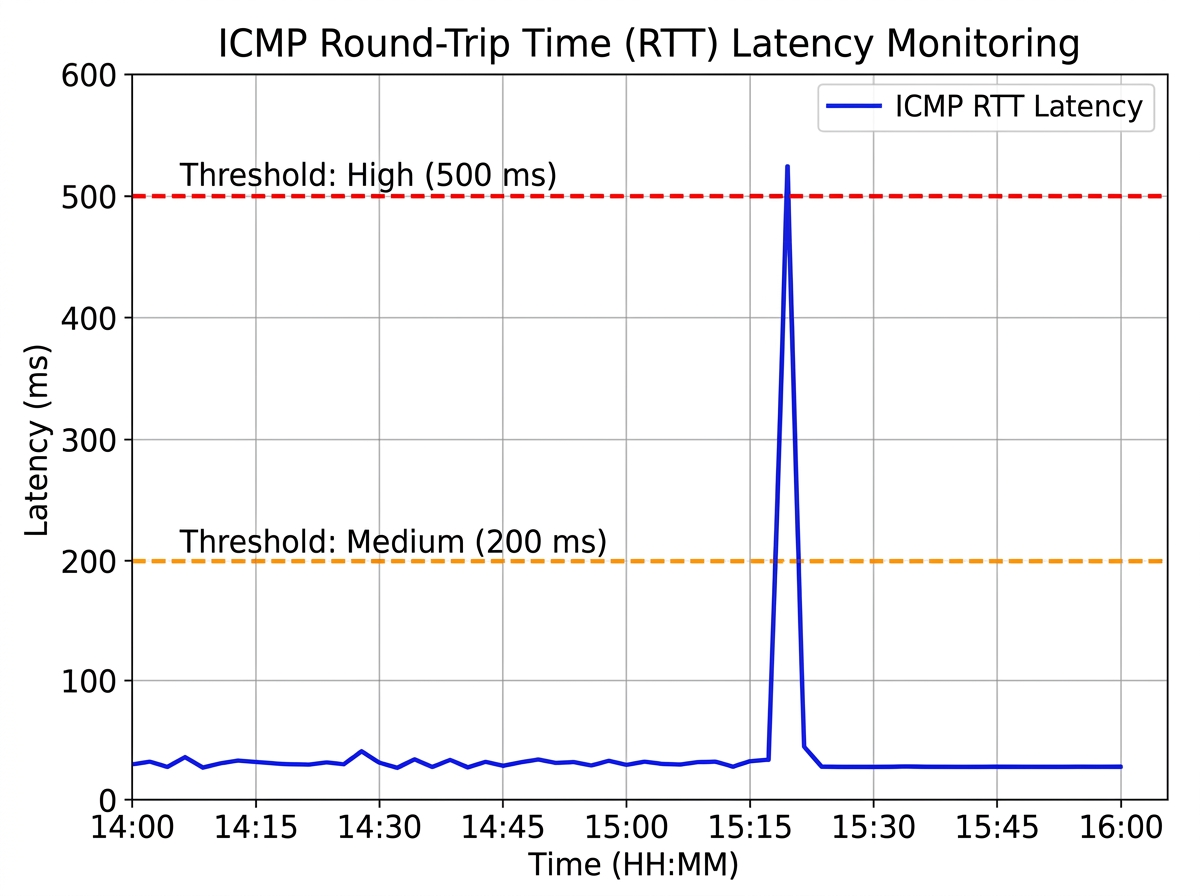
\includegraphics[width=\linewidth]{latency_trend.png}
    \caption{ICMP RTT latency (ms)}
    \label{fig:sub_latency}
\end{subfigure}
\hfill
\begin{subfigure}[b]{0.48\columnwidth}
    \centering
    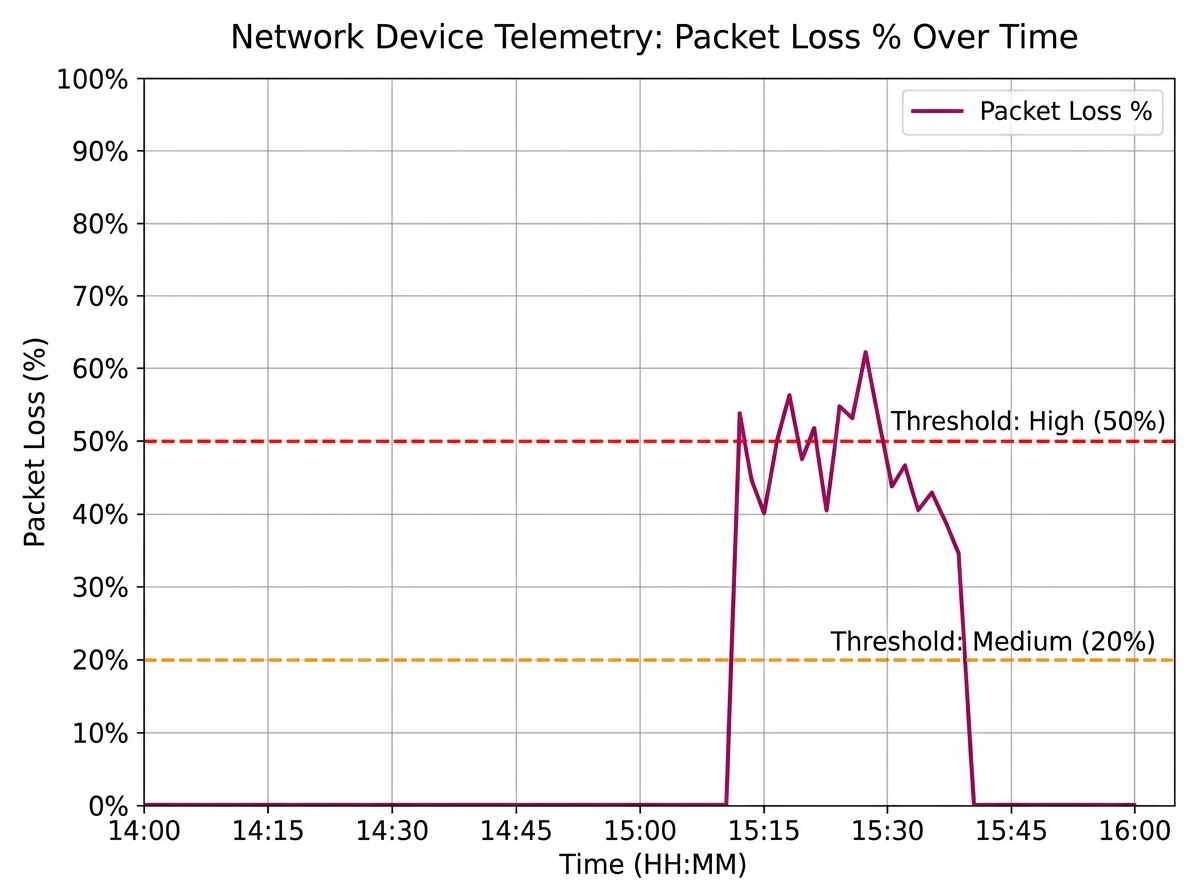
\includegraphics[width=\linewidth]{packet_loss.png}
    \caption{Packet loss (\%)}
    \label{fig:sub_loss}
\end{subfigure}
\caption{Historical telemetry trends captured by background Celery polling tasks and visualized via Recharts time-series components.}
\label{fig:telemetry_trends}
\end{figure}

\begin{figure}[htbp]
\centering
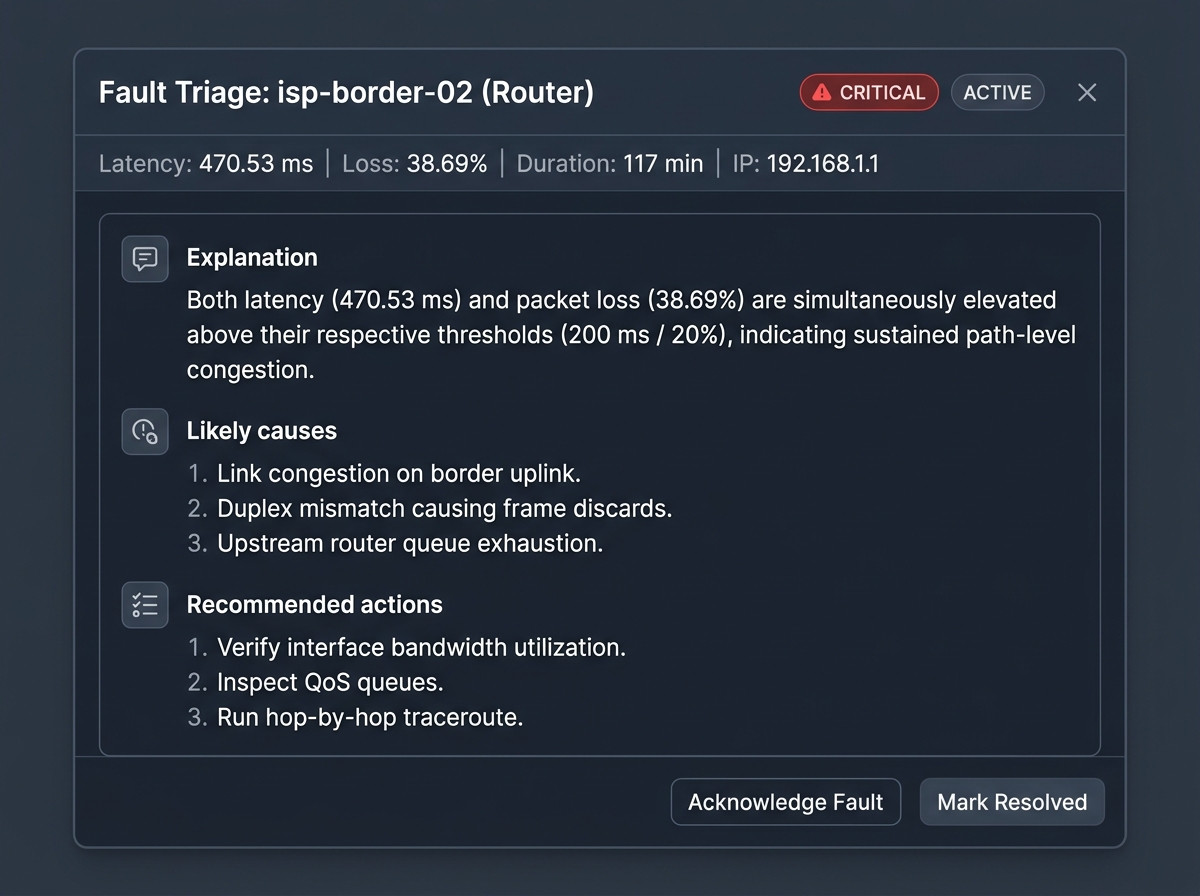
\includegraphics[width=\columnwidth]{fault_triage.png}
\caption{Operator triage interface displaying the fine-tuned LLM's structured diagnostic: \textit{Explanation}, \textit{Likely causes}, and \textit{Recommended actions} sections rendered inline within the fault detail modal.}
\label{fig:fault_triage}
\end{figure}

\subsection{LLM Inference Integration}

On fault creation, the Django backend asynchronously queues a Celery task that (i) constructs an inference prompt from the fault record's device context, metric snapshot, and fault type, (ii) submits the prompt to the locally hosted fine-tuned adapter (loaded via \texttt{transformers} + \texttt{peft}), and (iii) stores the generated triage text back to the Fault record. The React frontend polls the fault detail endpoint and renders the explanation once available, with a skeleton loading state in the interim. This asynchronous approach ensures that LLM inference latency (typically 2--6 seconds on a consumer GPU) does not block the operator interface or the monitoring pipeline.

% ============================================================
\section{Limitations \& Future Work}
\label{sec:limitations}

\subsection{Current Limitations}

\textbf{Simulated SNMP in Development.} The SNMP module in the current implementation supports real v1/v2c polling but was primarily validated against SNMP-simulated devices in the development environment. Production deployment against diverse enterprise switch and router firmware requires extended testing of OID compatibility and community string handling across vendor-specific MIBs.

\textbf{Single-Tenant Deployment.} The current SQLite-backed persistence layer limits horizontal scalability. Migration to PostgreSQL with connection pooling would be required for multi-tenant or high-device-count deployments.

\textbf{Edge Device Compute.} While the 1.5B-parameter model is significantly smaller than frontier models, inference on CPU-only edge gateways still requires 8--12 seconds per triage generation. Further quantization to 2-bit GPTQ or deployment via GGUF/llama.cpp runtimes would be required for genuinely latency-sensitive edge scenarios.

\textbf{Static Thresholds.} The fault detection engine uses manually configured static thresholds. Network behavior is inherently contextual: a 300\,ms RTT may be anomalous on a local LAN but acceptable on a trans-oceanic WAN segment. Adaptive threshold learning from historical baselines would improve alert precision.

\subsection{Future Directions}

\textbf{Retrieval-Augmented Generation (RAG).} Augmenting the LLM inference pipeline with a RAG module over device manuals, vendor advisories, and historical incident records would allow triage reports to reference device-specific configuration guidance and known firmware bugs, substantially improving actionability.

\textbf{Automated Remediation Script Execution.} The current system stops at generating recommended actions in natural language. Extending the pipeline to generate and optionally execute parameterized remediation scripts (e.g., interface resets via SSH, VLAN reconfiguration via NETCONF) would move the system toward autonomous network self-healing.

\textbf{Multi-Modal Telemetry.} Incorporating flow-level telemetry (NetFlow/IPFIX) and topology-aware graph embeddings alongside per-device metric snapshots would enable more precise root-cause attribution in shared-medium network segments.

\textbf{Continual Learning.} Operator feedback on generated triage reports (accept/reject/edit) could be used to construct an online preference dataset for DPO or RLHF-based continual adaptation, aligning the model to organization-specific remediation conventions over time.

% ============================================================
\section{Conclusion}
\label{sec:conclusion}

We have presented a unified AIOps platform that bridges the gap between raw network telemetry and actionable operator guidance through a combination of deterministic fault detection and domain-adapted generative AI. The monitoring subsystem provides production-grade asynchronous ICMP, SNMP, and HTTP probing with a rigorous fault lifecycle state machine. The NLP subsystem demonstrates that a 1.5B-parameter model fine-tuned via QLoRA on an 830-sample, carefully engineered dataset can achieve 100\% structural output compliance and 3$\times$ BLEU/ROUGE-L improvement over zero-shot baselines on network triage tasks, with robust generalization to out-of-domain compound fault scenarios. The integrated React dashboard delivers this capability to operators without requiring specialist network engineering knowledge at the point of alert triage. This work establishes a replicable blueprint for applying parameter-efficient fine-tuning to domain-specific operational AI assistants in resource-constrained deployment environments.

% ============================================================
\begin{thebibliography}{99}

\bibitem{chen2019outage}
J.\ Chen et al., ``Outage Prediction and Diagnosis for Cloud Service Systems,'' in \textit{Proc.\ WWW}, 2019, pp.\ 2803--2809.

\bibitem{luo2021ntam}
C.\ Luo et al., ``NTAM: Neighborhood-Temporal Attention Model for Disk Failure Prediction in Cloud Production Environments,'' in \textit{Proc.\ WWW}, 2021, pp.\ 1181--1191.

\bibitem{brown2020gpt3}
T.\ B.\ Brown et al., ``Language Models are Few-Shot Learners,'' in \textit{Advances in Neural Information Processing Systems (NeurIPS)}, vol.\ 33, 2020, pp.\ 1877--1901.

\bibitem{touvron2023llama2}
H.\ Touvron et al., ``Llama 2: Open Foundation and Fine-Tuned Chat Models,'' \textit{arXiv preprint arXiv:2307.09288}, 2023.

\bibitem{dettmers2023qlora}
T.\ Dettmers, A.\ Pagnoni, A.\ Holtzman, and L.\ Zettlemoyer, ``QLoRA: Efficient Finetuning of Quantized LLMs,'' in \textit{Advances in Neural Information Processing Systems (NeurIPS)}, vol.\ 36, 2023, pp.\ 10088--10115.

\bibitem{hu2022lora}
E.\ J.\ Hu et al., ``LoRA: Low-Rank Adaptation of Large Language Models,'' in \textit{Proc.\ ICLR}, 2022.

\bibitem{nagios}
E.\ Galstad, ``Nagios: System and network monitoring,'' \textit{Open Source Press}, 2008.

\bibitem{zabbix}
R.\ Olups, \textit{Zabbix 1.8 Network Monitoring}. Packt Publishing, 2010.

\bibitem{prometheus}
B.\ Rabenstein and J.\ Volz, ``Prometheus: A next-generation monitoring system,'' in \textit{Proc.\ USENIX LISA}, 2015.

\bibitem{dang2019aiops}
Y.\ Dang, Q.\ Lin, and P.\ Huang, ``AIOps: Real-World Challenges and Research Innovations,'' in \textit{Proc.\ ICSE: SEIP}, 2019, pp.\ 4--5.

\bibitem{zhao2020multivariate}
H.\ Zhao et al., ``Multivariate Time-Series Anomaly Detection via Graph Attention Network,'' in \textit{Proc.\ IEEE ICDM}, 2020, pp.\ 841--850.

\bibitem{le2023log}
V.-H.\ Le and H.\ Zhang, ``Log-based Anomaly Detection with Deep Learning: How Far Are We?'' in \textit{Proc.\ ICSE}, 2022, pp.\ 1--12.

\bibitem{ahmed2023recommending}
T.\ Ahmed et al., ``Recommending Root Cause and Mitigation for Cloud Incidents Using LLMs,'' in \textit{Proc.\ ESEC/FSE}, 2023.

\bibitem{chen2023empowering}
X.\ Chen et al., ``Empowering Practical Root Cause Analysis by Large Language Models for Cloud Incidents,'' \textit{arXiv preprint arXiv:2305.15778}, 2023.

\bibitem{qwen25}
Qwen Team, ``Qwen2.5 Technical Report,'' \textit{arXiv preprint arXiv:2412.15115}, 2024.

\bibitem{vonwerra2022trl}
L.\ von Werra et al., ``TRL: Transformer Reinforcement Learning,'' GitHub repository, \url{https://github.com/huggingface/trl}, 2022.

\bibitem{papineni2002bleu}
K.\ Papineni, S.\ Roukos, T.\ Ward, and W.-J.\ Zhu, ``BLEU: A Method for Automatic Evaluation of Machine Translation,'' in \textit{Proc.\ ACL}, 2002, pp.\ 311--318.

\bibitem{lin2004rouge}
C.-Y.\ Lin, ``ROUGE: A Package for Automatic Evaluation of Summaries,'' in \textit{Proc.\ ACL Workshop on Text Summarization Branches Out}, 2004, pp.\ 74--81.

\end{thebibliography}

\end{document}
